\SourcePage{223}{226}
\section{Passage through a potential barrier}

Consider the motion of a particle in a field of the type shown in Fig.~13. It
contains a \emph{potential barrier}: a region where the potential energy
$U(x)$ exceeds the particle's total energy $E$. In classical mechanics such a
barrier is impenetrable. In quantum mechanics, however, there is a nonzero
probability that the particle will pass ``through the barrier'' (this is also
called the \emph{tunnelling effect})\footnote{Examples of this kind were
already considered in Problems 2 and 4 of \S~25.}. If $U(x)$ meets the
conditions for the semiclassical approximation, the transmission coefficient
of the barrier can be found in general form. These conditions imply, in
particular, that the barrier is wide; consequently, its semiclassical
transmission coefficient is small.

\begin{figure}[ht]
\centering
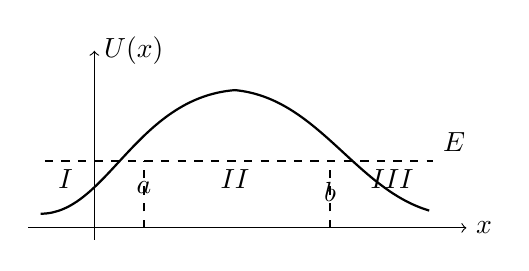
\begin{tikzpicture}[x=1.05cm,y=1.0cm]
  \draw[->] (-2.5,0)--(2.8,0) node[right] {$x$};
  \draw[->] (-1.7,-0.15)--(-1.7,2.25) node[right] {$U(x)$};
  \draw[dashed] (-2.3,.85)--(2.4,.85) node[above right] {$E$};
  \draw[thick] (-2.35,.18) .. controls (-1.55,.18) and (-1.2,1.65) .. (0,1.75)
    .. controls (1.0,1.65) and (1.45,.5) .. (2.35,.22);
  \draw[dashed] (-1.1,0)--(-1.1,.85) node[below=4pt] {$a$};
  \draw[dashed] (1.15,0)--(1.15,.85) node[below=4pt] {$b$};
  \node at (-2.05,.62) {$I$}; \node at (0,.62) {$II$}; \node at (1.9,.62) {$III$};
\end{tikzpicture}
\par\smallskip Fig. 13
\end{figure}

Before continuing the calculation, we solve an auxiliary problem. Suppose that
to the right of the turning point $x=b$, where

\SourcePage{224}{227}
$U(x)<E$, the semiclassical wave function is the travelling wave
\begin{equation}
 \psi=\frac{C}{\sqrt p}\exp\left(\frac{i}{\hbar}\int_b^x p\,dx+\frac{i\pi}{4}\right).
 \tag{50.1}
\end{equation}
We must find the wave function of the same state for $x<b$. We use the same
continuation around the complex $x$-plane as in \S~47.

Putting
\[
 E-U(x)\approx F_0(x-b),\qquad F_0>0,
\]
we rewrite (50.1) as
\[
 \psi(x)=\frac{C}{(2mF_0)^{1/4}}\frac1{(x-b)^{1/4}}
 \exp\left\{\frac{i}{\hbar}(2mF_0)^{1/2}
 \int_b^x\sqrt{x-b}\,dx+\frac{i\pi}{4}\right\}.
\]
Continue this expression from right to left along a semicircle in the upper
half-plane:
\[
 x-b=\rho e^{i\varphi},\qquad
 i\int_b^x\sqrt{x-b}\,dx=\frac23\rho^{3/2}
 \left(-\sin\frac{3\varphi}{2}+i\cos\frac{3\varphi}{2}\right),
\]
with $\varphi$ running from 0 to $\pi$. During this continuation $|\psi(x)|$
first decreases and then increases. At its end,
\[
 \psi(x)=\frac{C}{(2mF_0)^{1/4}}\frac1{(b-x)^{1/4}e^{i\pi/4}}
 \exp\left\{\frac1\hbar\int_x^b(2mF_0)^{1/2}\sqrt{b-x}\,dx+\frac{i\pi}{4}\right\}.
\]
We therefore obtain the correspondence rule\footnote{If the continuation
from right to left is instead made through the lower half-plane, $|\psi(x)|$
first increases and then decreases, becoming exponentially small on the
negative half-axis ($\varphi\to-\pi$). It would be illegitimate to retain this
small quantity against the exponentially large function (50.2). On the part
of the path where $\psi(x)$ is exponentially large, the inaccuracy of the
semiclassical approximation loses an exponentially small addition which, as
$\varphi\to-\pi$, could have grown into an exponentially large term and is
therefore likewise lost.}:
\begin{equation}
 \left.\frac{C}{\sqrt p}\exp\left\{\frac{i}{\hbar}\int_b^x p\,dx+
 \frac{i\pi}{4}\right\}\right|_{x>b}
 \longrightarrow
 \left.\frac{C}{\sqrt{|p|}}\exp\left\{\frac1\hbar
 \left|\int_b^x p\,dx\right|\right\}\right|_{x<b}.
 \tag{50.2}
\end{equation}

\SourcePage{225}{228}
This rule presupposes a particular wave in the classically allowed region---a
wave travelling to the right---and must be used specifically in passing from
that region into the classically forbidden one.

We return to the transmission coefficient of the barrier. Let a particle be
incident on it from region $I$, moving to the right. Beyond the barrier, in
region $III$, there is only the transmitted right-moving wave. Write it as
\begin{equation}
 \psi=\sqrt{\frac Dv}\exp\left(\frac{i}{\hbar}\int_b^x p\,dx+\frac{i\pi}{4}\right),
 \tag{50.3}
\end{equation}
where $v=p/m$ is the particle velocity and $D$ is the current density in the
wave. Rule (50.2) now gives, inside the barrier in region $II$,
\begin{equation}
 \psi=\sqrt{\frac D{|v|}}\exp\left(\frac1\hbar\left|\int_x^b p\,dx\right|\right)
 =\sqrt{\frac D{|v|}}\exp\left(\frac1\hbar\left|\int_a^b p\,dx\right|
 -\frac1\hbar\left|\int_a^x p\,dx\right|\right).
 \tag{50.4}
\end{equation}
Finally, application of (47.5) gives, before the barrier in region $I$,
\[
 \psi=2\sqrt{\frac Dv}\exp\left(\frac1\hbar\int_a^b|p|\,dx\right)
 \cos\left(\frac1\hbar\int_x^a p\,dx-\frac\pi4\right).
\]
If we set
\begin{equation}
 D=\exp\left(-\frac2\hbar\int_a^b|p|\,dx\right),
 \tag{50.5}
\end{equation}
this becomes
\[
 \begin{split}
 \psi&=\frac2{\sqrt v}\cos\left(\frac1\hbar\int_a^x p\,dx+\frac\pi4\right)\\
 &=\frac1{\sqrt v}\exp\left(\frac{i}{\hbar}\int_a^x p\,dx+\frac{i\pi}{4}\right)
 +\frac1{\sqrt v}\exp\left(-\frac{i}{\hbar}\int_a^x p\,dx-\frac{i\pi}{4}\right).
 \end{split}
\]

\SourcePage{226}{229}
The first term (which tends to the plane wave $\psi\sim e^{ipx/\hbar}$ as
$x\to-\infty$) describes the incident wave, and the second the reflected
wave. Our normalization assigns unit current density to the incident wave.
Thus $D$, the current density in the transmitted wave, is precisely the
required barrier transmission coefficient. Formula (50.5) is applicable only
when its exponent is large and $D$ itself is consequently small\footnote{The
exponential smallness of $D$ also explains why the incident and reflected
waves in region $I$ have equal amplitudes: their exponentially small
difference is lost in the semiclassical approximation.}.

So far we have assumed that $U(x)$ satisfies the semiclassical condition
throughout the barrier, apart from the immediate neighbourhoods of the
turning points. In practice one often meets barriers whose potential-energy
curve rises so sharply on one side that the semiclassical approximation
fails. The leading exponential factor in $D$ remains the one in (50.5), but
the pre-exponential factor (unity in (50.5)) changes. To calculate it, one
must in principle find the exact wave function in the non-semiclassical
region and match it to the semiclassical wave function within the barrier.

\begin{center}\textbf{P r o b l e m s}\end{center}

\ProblemHeading{1.} Find the transmission coefficient of the barrier in
Fig.~14: $U(x)=0$ for $x<0$, $U(x)=U_0-Fx$ for $x>0$. Calculate only its
exponential factor.

\SolutionHeading Direct calculation gives
\[
 D\sim\exp\left[-\frac{4\sqrt{2m}}{3\hbar F}(U_0-E)^{3/2}\right].
\]

\ProblemHeading{2.} Find the probability that a particle of zero angular
momentum escapes from the spherically symmetric potential well
$U(r)=-U_0$ for $r<r_0$, $U(r)=\alpha/r$ for $r>r_0$ (Fig.~15)\footnote{This
problem was first considered by G.~F.~Gamow (1928), and by
$R. W. Gurney$ and $E. U. Condon$ (1929), in connection with the theory of
radioactive $\alpha$-decay.}.

\SolutionHeading A spherically symmetric problem reduces to a
one-dimensional one, so the preceding formulas apply. Hence
\[
 w\sim\exp\left[-\frac2\hbar\int_{r_0}^{\alpha/E}
 \sqrt{2m\left(\frac\alpha r-E\right)}\,dr\right].
\]

\SourcePage{227}{230}
Evaluation of the integral gives
\[
 w\sim\exp\left\{-\frac{2\alpha}{\hbar}\sqrt{\frac{2m}{E}}
 \left[\arccos\sqrt{\frac{Er_0}{\alpha}}-
 \sqrt{\frac{Er_0}{\alpha}\left(1-\frac{Er_0}{\alpha}\right)}\right]\right\}.
\]

\begin{figure}[ht]
\centering
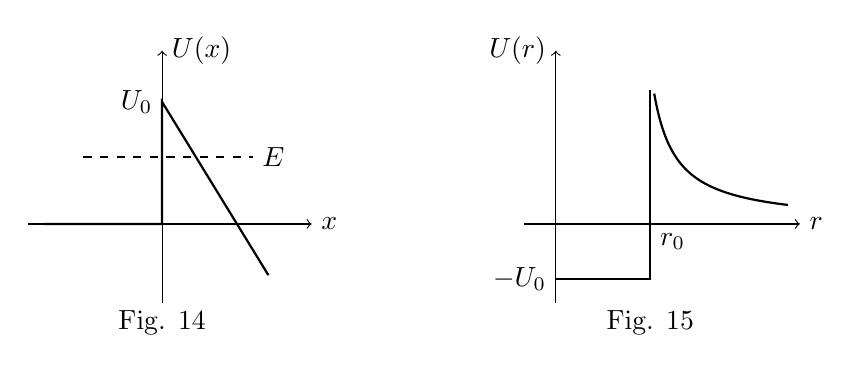
\begin{tikzpicture}[x=1cm,y=1cm]
 \begin{scope}[xshift=-3.1cm]
  \draw[->] (-1.7,0)--(1.9,0) node[right] {$x$};
  \draw[->] (0,-1)--(0,2.2) node[right] {$U(x)$};
  \draw[thick] (-1.5,0)--(0,0)--(0,1.55)--(1.35,-.65);
  \draw[dashed] (-1,.85)--(1.15,.85) node[right] {$E$};
  \node[left] at (0,1.55) {$U_0$};
  \node at (0,-1.25) {Fig. 14};
 \end{scope}
 \begin{scope}[xshift=3.1cm]
  \draw[->] (-1.6,0)--(1.9,0) node[right] {$r$};
  \draw[->] (-1.2,-1)--(-1.2,2.2) node[left] {$U(r)$};
  \draw[thick] (-1.2,-.7)--(0,-.7)--(0,1.7);
  \draw[thick,domain=.05:1.75,samples=80] plot (\x,{.48/(\x+.24)});
  \node[left] at (-1.2,-.7) {$-U_0$}; \node[below right] at (0,0) {$r_0$};
  \node at (0,-1.25) {Fig. 15};
 \end{scope}
\end{tikzpicture}
\end{figure}

As $r_0\to0$, this formula tends to
\[
 w\sim\exp\left(-\frac{\pi\alpha}{\hbar}\sqrt{\frac{2m}{E}}\right)
 =\exp\left(-\frac{2\pi\alpha}{\hbar v}\right).
\]
These formulas require a large exponent, i.e. $\alpha/\hbar v\gg1$. As it
should, this agrees with the semiclassical condition (49.11) for motion in a
Coulomb field.

\ProblemHeading{3.} The field $U(x)$ consists of two symmetric potential
wells ($I$ and $II$ in Fig.~16), separated by a barrier. Were the barrier
impenetrable, there would be energy levels belonging to motion in one well or
the other, with identical values for both wells. Passage through the barrier
splits each such level into two nearby levels, corresponding to states in
which the particle moves in both wells. Find the splitting, assuming that
$U(x)$ is semiclassical.

\begin{figure}[ht]
\centering
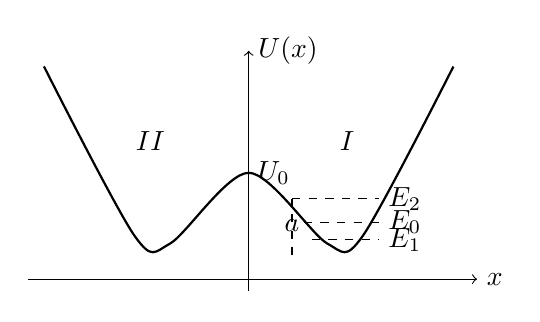
\begin{tikzpicture}[x=1cm,y=1cm]
 \draw[->] (-2.8,0)--(2.9,0) node[right] {$x$};
 \draw[->] (0,-.15)--(0,2.9) node[right] {$U(x)$};
 \draw[thick] plot[smooth] coordinates {(-2.6,2.7)(-1.45,.55)(-1,.45)(0,1.35)(1,.45)(1.45,.55)(2.6,2.7)};
 \draw[dashed] (0.55,.3)--(0.55,1.02) node[below=4pt] {$a$};
 \draw[dashed] (.55,1.02)--(1.65,1.02) node[right] {$E_2$};
 \draw[dashed] (.7,.72)--(1.65,.72) node[right] {$E_0$};
 \draw[dashed] (.8,.5)--(1.65,.5) node[right] {$E_1$};
 \node at (-1.25,1.75) {$II$}; \node at (1.25,1.75) {$I$}; \node[right] at (0,1.35) {$U_0$};
\end{tikzpicture}
\par\smallskip Fig. 16
\end{figure}

\SolutionHeading Neglecting passage through the barrier, construct an
approximate solution of the Schrödinger equation from a semiclassical wave
function $\psi_0(x)$ describing motion, at some energy $E_0$, in one well
(say well $I$). It decays exponentially on both sides of that well, and is
normalized so that the integral of $\psi_0^2$ over well $I$ is unity. Once
the small tunnelling probability is admitted, $E_0$ splits into $E_1$ and
$E_2$. The appropriate zeroth-order wave functions are the symmetric and
antisymmetric combinations of $\psi_0(x)$ and $\psi_0(-x)$:
\begin{equation}
 \psi_1(x)=\frac1{\sqrt2}[\psi_0(x)+\psi_0(-x)],\qquad
 \psi_2(x)=\frac1{\sqrt2}[\psi_0(x)-\psi_0(-x)]. \tag{1}
\end{equation}

\SourcePage{228}{231}
In well $I$, $\psi_0(-x)$ is negligibly small compared with $\psi_0(x)$;
in well $II$ the reverse is true. The product $\psi_0(x)\psi_0(-x)$ is thus
negligible everywhere, and (1) are normalized so that the integrals of their
squares over wells $I$ and $II$ are unity.

Write the Schrödinger equations
\[
 \psi_0''+\frac{2m}{\hbar^2}(E_0-U)\psi_0=0,\qquad
 \psi_1''+\frac{2m}{\hbar^2}(E_1-U)\psi_1=0.
\]
Multiply the first by $\psi_1$, the second by $\psi_0$, subtract, and
integrate over $0<x<\infty$. Since at $x=0$,
$\psi_1=\sqrt2\psi_0$, $\psi_1'=0$, and
\[
 \int_0^\infty\psi_0\psi_1\,dx\approx\frac1{\sqrt2}
 \int_0^\infty\psi_0^2\,dx=\frac1{\sqrt2},
\]
we obtain
\[
 E_1-E_0=-\frac{\hbar^2}{m}\psi_0(0)\psi_0'(0).
\]
The same calculation gives $E_2-E_0$ with the opposite sign. Therefore
\[
 E_2-E_1=\frac{2\hbar^2}{m}\psi_0(0)\psi_0'(0).
\]
Using (47.1), with the coefficient $C$ from (48.3), we find
\[
 \psi_0(0)=\sqrt{\frac{\omega}{2\pi v_0}}
 \exp\left(-\frac1\hbar\int_0^a|p|\,dx\right),\qquad
 \psi_0'(0)=\frac{mv_0}{\hbar}\psi_0(0),
\]
where $v_0=\sqrt{2(U_0-E_0)/m}$. Hence
\[
 E_2-E_1=\frac{\omega\hbar}{\pi}
 \exp\left(-\frac1\hbar\int_{-a}^a|p|\,dx\right),
\]
where $a$ is the turning point for the energy $E_0$ (see Fig.~16).

\ProblemHeading{4.} Find the exact transmission coefficient $D$, without
assuming it small, for the parabolic barrier $U(x)=-kx^2/2$
($E. C. Kemble$, 1935)\footnote{The solution also applies to passage close
enough to the top of any barrier whose $U(x)$ is quadratic near its maximum.}.

\SolutionHeading For any $k$ and $E$, the motion is semiclassical at
sufficiently large $|x|$, where
\[
 p=\sqrt{2m\left(E+\frac12kx^2\right)}\approx x\sqrt{mk}
 +E\sqrt{\frac mk}\frac1x,
\]
and the asymptotic solution of the Schrödinger equation has the form
\[
 \psi=\operatorname{const}\cdot\xi^{\pm i\varepsilon-1/2}
 \exp(\pm i\xi^2/2),
\]

\SourcePage{229}{232}
where
\[
 \xi=x\left(\frac{mk}{\hbar^2}\right)^{1/4},\qquad
 \varepsilon=\frac E\hbar\sqrt{\frac mk}.
\]
We require the solution that, as $x\to+\infty$, contains only the wave
transmitted through the barrier, travelling from left to right. Put
\begin{align}
 \psi&=B\xi^{i\varepsilon-1/2}\exp(i\xi^2/2)
 &&\text{for }x\to\infty, \tag{1}\\
 \psi&=(-\xi)^{-i\varepsilon-1/2}\exp(-i\xi^2/2)
 +A(-\xi)^{i\varepsilon-1/2}\exp(i\xi^2/2)
 &&\text{for }x\to-\infty. \tag{2}
\end{align}
The first term in (2) is incident and the second reflected (a wave propagates
in the direction in which its phase increases). The relation between $A$ and
$B$ follows because the asymptotic expression for $\psi$ is valid throughout
the sufficiently distant part of the complex $\xi$-plane. Follow (1) around
a large semicircle of radius $\rho$ in the upper half-plane:
\[
 \xi=\rho e^{i\varphi},\qquad
 i\xi^2=\rho^2(-\sin2\varphi+i\cos2\varphi),
\]
where $\varphi$ runs from 0 to $\pi$. After this continuation, (1) becomes
the second term in (2), with
\begin{equation}
 A=B(e^{i\pi})^{i\varepsilon-1/2}=-iBe^{-\pi\varepsilon}. \tag{3}
\end{equation}
On the portion $\pi/2<\varphi<\pi$, where
$|\exp(i\xi^2/2)|$ is exponentially large, the exponentially small quantity
which should produce the first term in (2) is lost\footnote{Continuation
through the lower half-plane would not determine $A$: on
$-\pi<\varphi<-\pi/2$, adjoining the left endpoint where (2) applies, the
term containing $\exp(i\xi^2/2)$ is exponentially small compared with the
term containing $\exp(-i\xi^2/2)$.}.

With the incident-wave normalization chosen in (2), particle-number
conservation reads
\begin{equation}
 |A|^2+|B|^2=1. \tag{4}
\end{equation}
Equations (3) and (4) give the desired coefficient
\[
 D=|B|^2=1/(1+e^{-2\pi\varepsilon}).
\]
This holds for every $E$. If $E$ is negative and large in magnitude,
$D\approx e^{-2\pi|\varepsilon|}$, in agreement with (50.5). For $E>0$,
\[
 R=1-D=1/(1+e^{2\pi\varepsilon})
\]
is the above-barrier reflection coefficient.
